
This section will cover how to install and use the Protégé plugin developed to allow using the techniques presented in the thesis.

\section{Installation}

The Protégé plugin can either be compiled and packaged form source, or is available at \url{https://github.com/rolandbernard/protege-weakening/releases}. If you desire to compile the plugin from source, you will need a Java 11 JDK and the Maven tool. If you have both of these, you can execute the following command to package the plugin, and thereafter, find the bundled JAR file in \inlinecode{target/protege-weakening-X.X.X.jar}.

\begin{lstlisting}
git clone https://github.com/rolandbernard/protege-weakening
cp protege-weakening
mvn clean compile package
\end{lstlisting}

The JAR file of the plugin must be placed into the plugin folder of Protégé. The location of this folder will vary depending on the platform and configuration of Protégé. In a Linux based environment for example it, will most likely be located in \inlinecode{\$HOME/.Protege/plugins/}. After copying the JAR file of the plugin into this folder, the plugin will automatically be loaded and initialized the next time Protégé is started. Note that the plugin will require at least Java 11 and Protégé version 5.6.1. The plugin may work for some older Protégé versions, but this has not been tested.

\section{Using the Menu}

\begin{figure}[htbp]
  \centering
  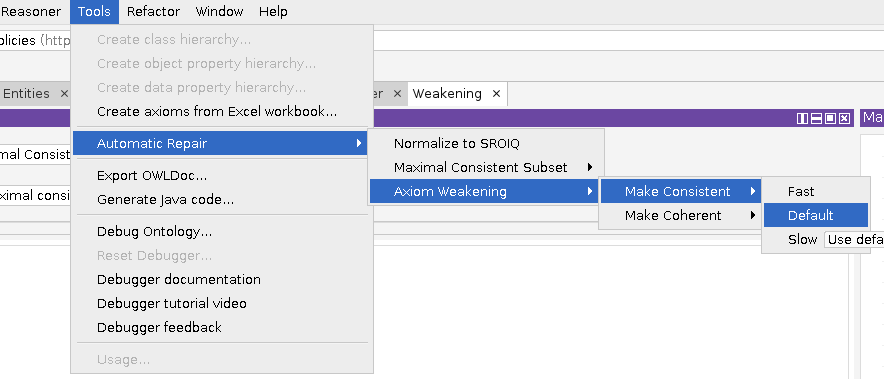
\includegraphics[width=\textwidth]{resources/protege-guide-menu.png}
  \caption{The menu items added by the plugin in Protégé.}
\end{figure}

The easiest way to use the plugin is by using the added menu items in the ``Tools'' section of the top menu. There are three main menu items. The ``Normalize to SROIQ'' entry will execute the normalization of the ontology that has also been used for the evaluation in the thesis. This will transform all OWL 2 axioms into axioms that more directly correspond to \SROIQ. Note that doing this is not required for starting the repair algorithms, since the axiom weakening operator implemented in the plugin has been extended to handle all OWL 2 axioms.

The next two menu items are for applying two different automatic repair algorithms. For each of them, there is the option of select between making the ontology only consistent, or making it also coherent. Note that when selecting coherence as the goal, the repairs will likely be slower, also because computing coherence is more expensive, at least using the way it is implemented for the plugin. The first repair method, used with the item ``Maximal Consistent Subset'', will select some randomly sampled maximal consistent subset. The second repair method, ``Axiom Weakening'', on the other hand, uses the axiom weakening based repair algorithm. Note that for each of these algorithms, there is also a choice between ``Fast'', ``Default'', or ``Slow''. These are some presets that make different choices of how to configure the repair algorithms. As their name suggests, they mainly consider options that have an impact on the performance of the algorithm. To have greater control over these parameters, use the automatic repair view.

\section{Using the Automatic Repair View}

\begin{figure}[htbp]
  \centering
  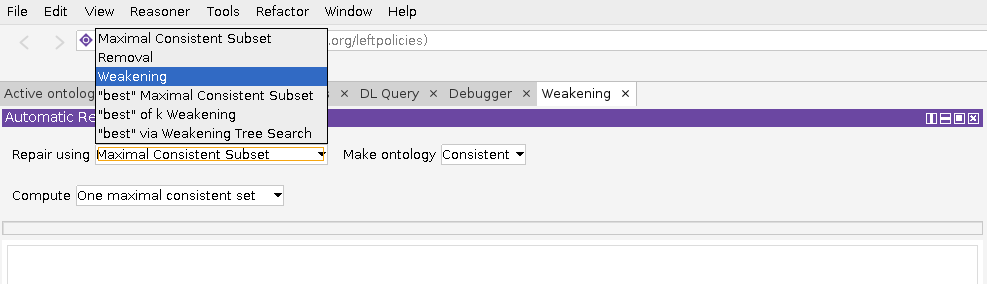
\includegraphics[width=\textwidth]{resources/protege-guide-algorithms.png}
  \caption{The automatic repair view added to Protégé. Showing the selection of possible algorithms.}
\end{figure}

The automatic repair view can be accessed in ``Window'' > ``Views'' > ``Ontology views'' > ``Automatic Repair''. It allows the user to select between a number of different repair algorithms. The one using axioms weakening and the one using a maximal consistent subset are the same as the ones accessible through the menu. The repair by removal is similar to the axiom weakening based repair, but the axioms are always removed instead of being weakened. The remaining three algorithms are all trying to optimize the IIC of the resulting repairs. For ``'best' Maximal Consistent Subset'' and ``best' of k Weakening'' this is done by sampling repairs using, respectively, maximal consistent subsets or axiom weakening, and then selecting from those the one that has the largest inferred call hierarchy. The algorithm used when selection ``'best' via Weakening Tree Search'', on the other hand, uses a Monte-Carlo tree search based approach to find the ontology with the largest inferred class hierarchy. Note that these last three repairs are significantly slower, both because they need to compute multiple repairs, and because they have to compute the inferred class hierarchy for each of them.

\begin{figure}[htbp]
  \centering
  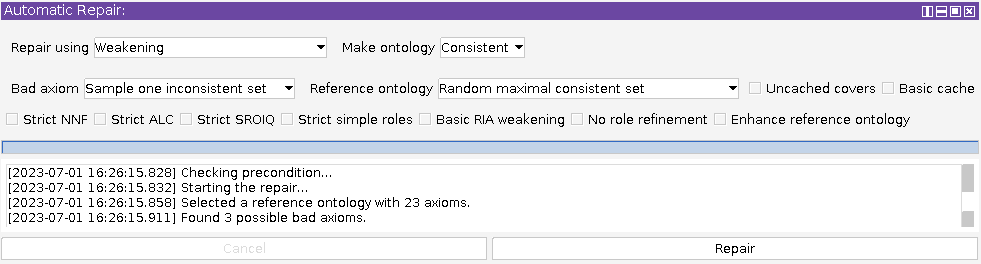
\includegraphics[width=\textwidth]{resources/protege-guide-config.png}
  \caption{The automatic repair view added to Protégé. Showing the different parameters that can be configured for the axiom weakening based repair method.}
  \label{fig:protege-guide-config}
\end{figure}

For each of these repair algorithms a number of different configuration option are made available to the user. \Cref{fig:protege-guide-config} shows the parameters that may be configured for the axiom weakening based repair algorithm. This includes different approaches for selecting reference ontologies and bad axioms. There are some options that allow using stricter checks, such as only allowing negation normal form, or only \ALC axioms and concepts. Further, there are some parameters that simplify the refinement of roles and one that chooses to not modify the axioms of the reference ontology.

To start the repair, use the ``Repair'' button at the bottom of the view. Some information about the running repair will be printed to the text output. While the repair is running, it can be interrupted by using the ``Cancel'' button that will become enabled whenever a repair is running. If a repair is cancelled, no change will be made to the ontology in Protégé. As soon as the repair completes on the other hand, the changes will be applied to the active ontology.

\section{Using the Manual Weakening View}

\begin{figure}[htbp]
  \centering
  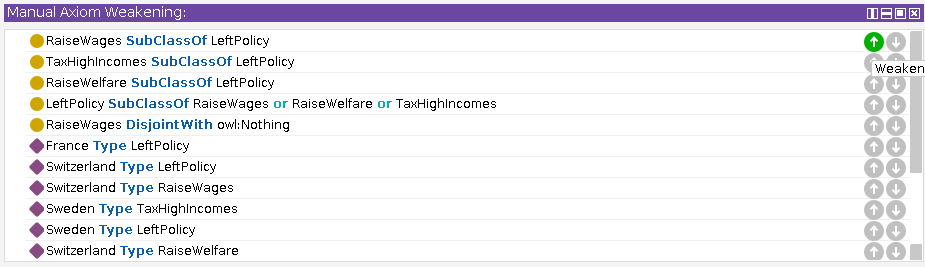
\includegraphics[width=\textwidth]{resources/protege-guide-list.png}
  \caption{The manual axiom weakening list added to Protégé. Use the buttons next to the axioms to weaken or strengthen the axioms.}
\end{figure}

The last view implemented by the plugin, and accessible under ``Window'' > ``Views'' > ``Ontology views'' > ``Manual Axiom Weakening'', allows for manually selecting which axioms to refine. The view shows a list of all axioms in the currently active ontology. The axioms are sorted by how frequently they appear in randomly sampled minimal inconsistent subsets. The axioms appearing the most often are shown at the top of the list. This means, that the axioms that would be chosen for weakening by the automatic repair algorithms are the ones appearing first in the list. Next to each axiom are two buttons, one with an upwards and one with a downwards arrow. These can be used to, respectively compute the axiom weakenings or axiom strengthening operator for that axiom.

\begin{figure}[htbp]
  \centering
  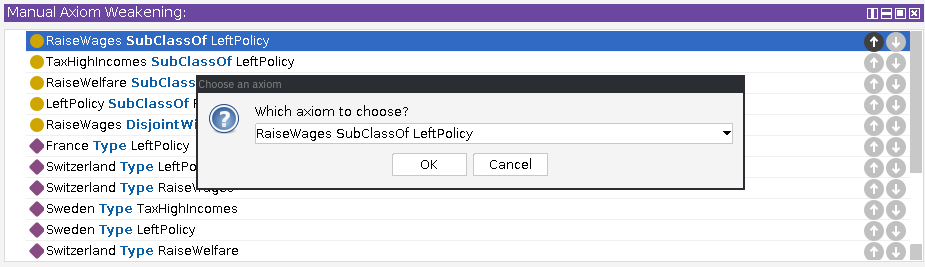
\includegraphics[width=\textwidth]{resources/protege-guide-replace.png}
  \caption{The selection of which refined axiom to use for replacing the original axiom, for the manual axiom weakening list added to Protégé.}
\end{figure}

Pressing one of these buttons will bring up a selection dialogue showing the results of the axiom weakening or strengthening operator. The user may then select from the presented choices one axiom and click ``Ok''. The original axiom will be removed from the ontology and replaced with the selected axiom. If the ``Cancel'' button is used on the other hand, no change will be made to the ontology.

